\documentclass[a4paper]{article}

\usepackage{fullpage}
\usepackage{graphicx}
\usepackage{url}
\usepackage{hyperref}
\usepackage{acronym}
\usepackage{paralist}
\usepackage{amsmath}
\usepackage{lipsum}
\usepackage{booktabs}
\usepackage{float}
\usepackage[ruled,vlined]{algorithm2e}


% ----------------------------------------------------------------------------
% Start the document
%
\begin{document}


\begin{centering}
~~~~~~~~~~~~~\\[-20mm]

  {
  \bfseries Master Degree in Computer Science\\[3mm]
  Web Architectures\\[3mm]
  AA 2014-2015
  }\\[1mm]


  \vspace{0.5cm}
  {
  \Large \bfseries{Java Enterprise Application} \par
  }
  {
  \small \bfseries{Project report} \par
  }
  \vspace{0.2cm}

  {Davide Spadini (id 164393)}

  \vspace{0.3cm}
\end{centering}



\section{Introduction}\label{introduction}
With this project I want to implement a \emph{Java Enterprise Application} that simulates the website of a Bank, enabling the user to check the its account, make a transaction to another client, withdraw or refill money from its account.

The application is divided in 3 parts:
\begin{compactitem}
  \item \textbf{Web Tier} Containing all the JSF pages and the Managed Beans
  \item \textbf{Business Tier} Containing the entity class, 2 stateless beans and 1 stateful bean
  \item \textbf{Persistent Tier} Database that contains all the users
\end{compactitem}

The Web Tier runs on Tomcat, the last two on Wildfly instead.

\section{Use Case and Class Diagram}
\label{sec:req_analysis}
The application can be used by an ``administrator'' or a ``user'': the first one can add or delete a new user and he has the complete list of them; the second one has associated a checking account and a credit card, he can make a bank transaction to another client, he can withdraw/refill money from/to its checking account or credit card. The complete Use Case Diagram is shown in Figure~\ref{fig:use_case_diagram}

\begin{figure}[ht]
  \centering
  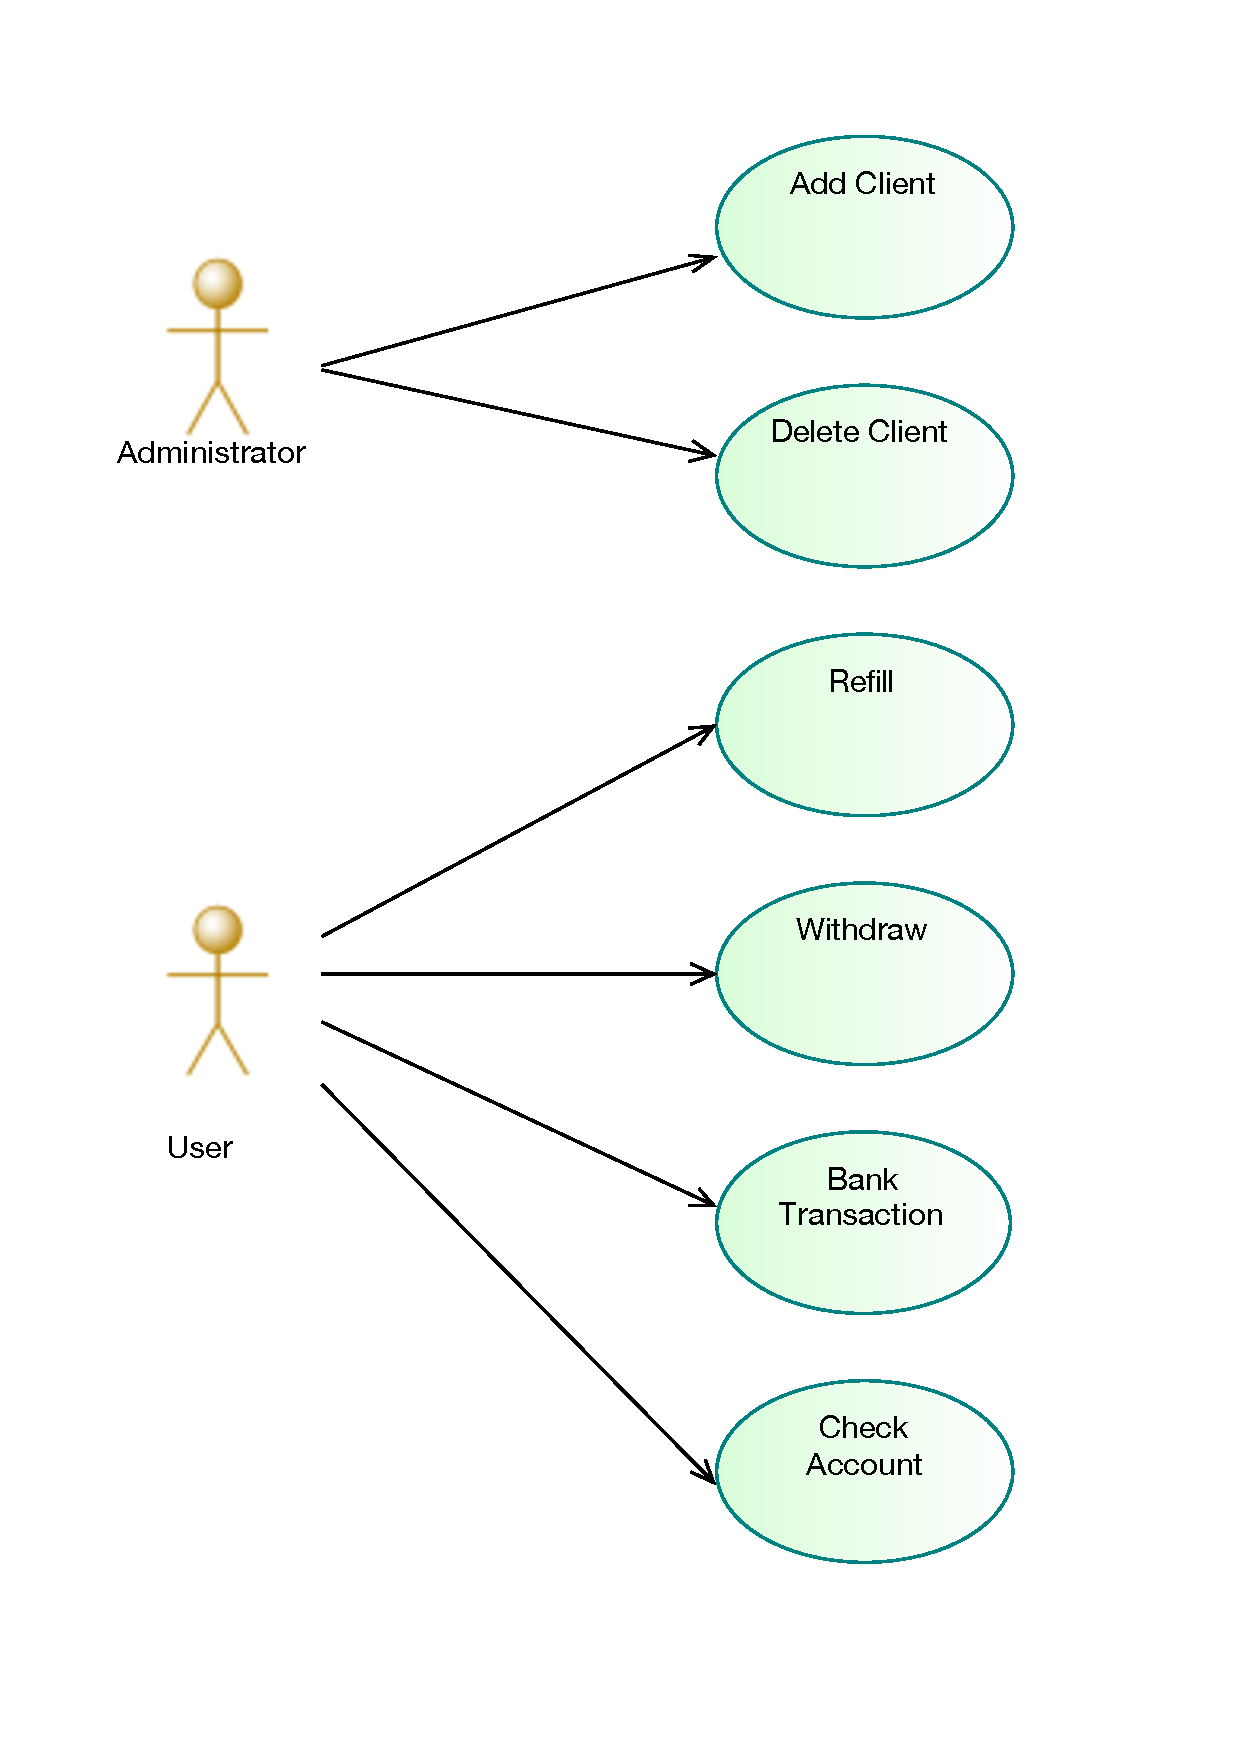
\includegraphics[keepaspectratio=true, width=5cm]{use_case_diagram}\caption{Use case Diagram.}
  \label{fig:use_case_diagram}
\end{figure}

\begin{figure}[ht]
  \centering
  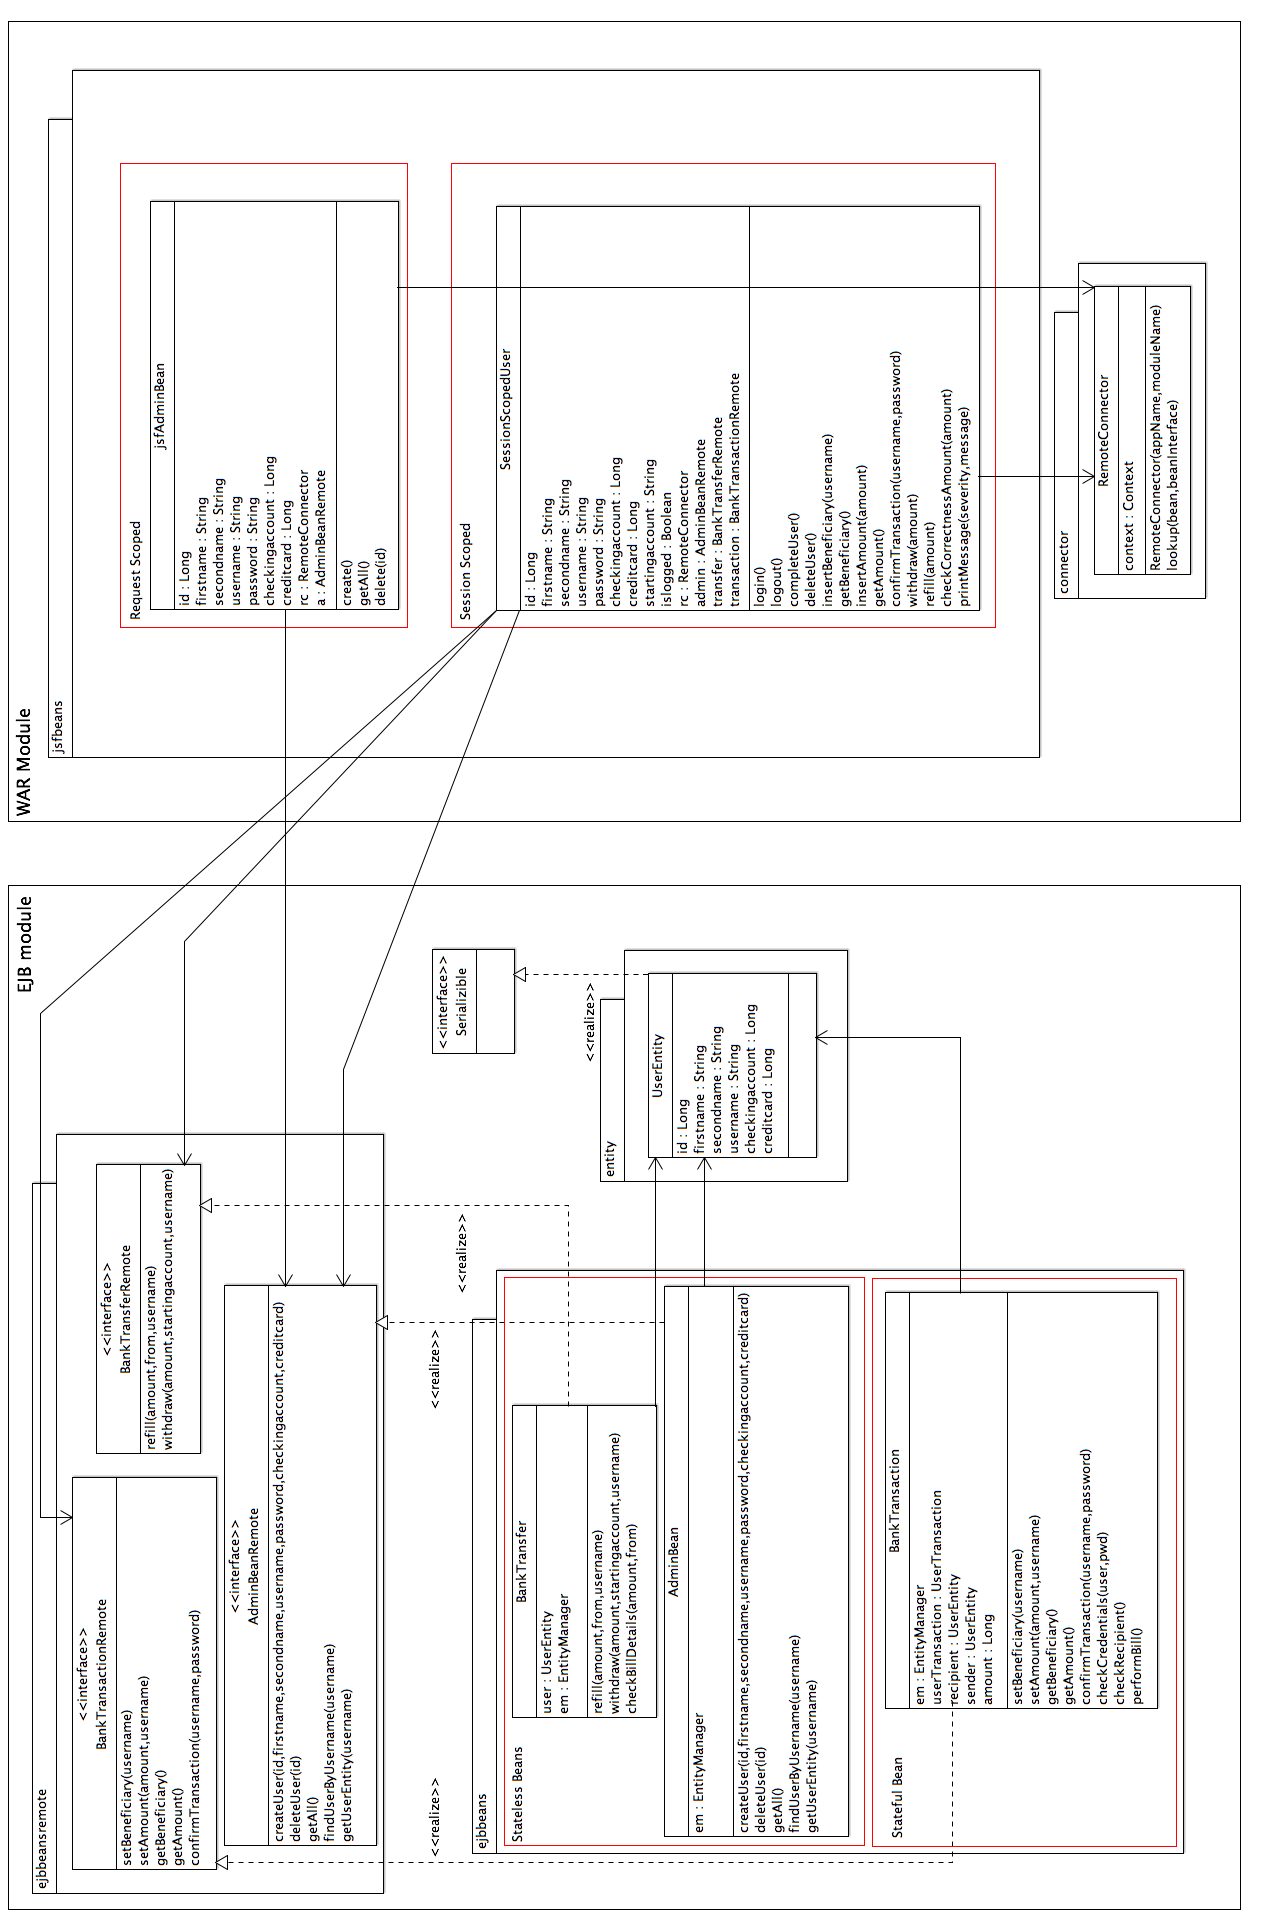
\includegraphics[keepaspectratio=true, width=\textwidth, height=\textheight]{ClassDiagram2.png}\caption{Use case Diagram.}
  \label{fig:classdiagram}
\end{figure}

\section{Usage} % (fold)
\label{sec:usage}

Processes are launched virtually together. Identification number $pid$ and size of the network $n$ are specified as command line parameters. In order to run a simulation, it is sufficient to launch $n$ instances of the following command on different shells:

\verb|python consensus.py <pid> <n> [<missing_assumption>]|
\\

The third parameter is optional and it is used to specify the assumption to be broken. Six choices are given, namely \emph{perfect\_channel}, \emph{partially\_async}, \emph{not\_byzantine}, \emph{max\_failures}, \emph{failure\_detector} and \emph{fully\_connected}. Their meaning and consequences are described below in Sect.\,\ref{sec:program_evaluation}.\newline
Routing tables for both the node and the failure detector are created automatically, then the oracle is initialized and nodes start to exchange the messages needed by the failure detector protocol. To start the consensus protocol it is sufficient to press \emph{Enter} on every process.

% section usage (end)

\section{Program architecture} % (fold)
\label{sec:program_architecture}

Our implementation assumes that the following properties hold:
\begin{compactitem}
  \item \textbf{Perfect Channels} \cite{models}
    \begin{compactitem}
      \item \textbf{Validity - Reliable delivery} A message sent by a correct process will be eventually received by the recipient.
      \item \textbf{Integrity - No duplication} No message is delivered to a process more than once.
      \item \textbf{Integrity - No creation} Every delivered message must have been sent by some process.
    \end{compactitem}
  \item \textbf{Partially asynchronous channels} The channel is \emph{infinitely often} synchronous.
  \item \textbf{Fully-connected graph} Each process can send messages to every other.
  \item \textbf{Failure by crash} Processes can fail only by crash, excluding byzantine behaviors.
  \item \textbf{Bounded failures} At most $f < n / 2$ processes can fail. This bound is imposed by the failure detector protocol we chose.
  \item \textbf{Failure detector $\diamond{}S$} There exists an oracle that provides hints about which processes are \emph{operational} or \emph{crashed} and that satisfies the following properties:
  \begin{compactitem}
    \item \textbf{Strong Completeness} Eventually \emph{every} faulty process is permanently suspected by \emph{every} correct process.
    \item \textbf{Eventual Weak Accuracy} Eventually \emph{some} correct process is never suspected by \emph{any} correct process.
  \end{compactitem}
\end{compactitem}

The program is divided in two main parts: the failure detector class and the consensus class.

\paragraph{Failure detector}
The implementation of the failure detector is based on the work of Larrea et al. \cite{larrea2013}, in particular the ``Wait-free $\diamond{}S$ Algorithm''.
%FIXME
\begin{quote}
The algorithm works in a system in which up to $n - 1$ processes can fail (i.e. it is wait free). This algorithm guarantees that all the correct processes eventually converge on the leader process $p_{leader}$ as a common correct process. This property trivially allows the algorithm to provide the eventual-weak accuracy required by $\diamond{}S$: eventually, $p_{leader}$ will not be suspected by any correct process. The strong completeness property of $\diamond{}S$ is achieved simply by making every process $p_i$ suspect all processes in the system except $p_{leader}$.
\end{quote}

The pseudo-code of the algorithm is shown in \textbf{Algorithm 1}.

\begin{algorithm}[H]
  \SetKwProg{Upon}{upon}{ do}{end}
  \SetKwProg{Every}{every}{ do}{end}
  \SetKwFunction{Send}{send}
  \SetKwFunction{Receive}{receive}

  \Upon{init}{
  $trusted_i \leftarrow 1$\;
  \ForEach{$j \in \{1, \dots, i - 1 \}$}{$\Delta_{i,j} \leftarrow$ default timeout}
  }
  \tcp{Task 1}
  \Every{default period}{
    \If{$trusted_i = i$}{
        \Send{I-AM-THE-LEADER} \KwTo $p_{i+1}, \dots, p_n$
    }
  }
  \tcp{Task 2}
  \Upon{$trusted_i < i$ {\bf and}\\
        (not \Receive{I-AM-THE-LEADER} from $p_{trusted_i}$ in the last $\Delta_{i, trusted_i}$ time units)}{
    $trusted_i \leftarrow trusted_i + 1$
  }
  \tcp{Task 3}
  \Upon{\Receive{I-AM-THE-LEADER} from $p_j$ {\bf and} $j < trusted_i$}{
    $trusted_i \leftarrow j$\;
    $\Delta_{i,j} \leftarrow \Delta_{i,j} + 1$
  }
 \caption{Failure detector algorithm executed by every process $p_i$}
\end{algorithm}
The failure detector has a local variable $trusted$ which is the guess of the correct process. At the beginning of the execution, it is initialized to $1$, meaning that $p_1$ is the current leader.
As the system evolves, $trusted_i$ eventually holds the lowest \emph{id} among those of the processes that have not failed, i.e. the leader.

The leader $p_{leader}$ periodically sends a \emph{I-AM-THE-LEADER} to the processes $p_i$ such that $i > leader$. In fact, $p_j$ can become the leader only if every $p_k$ such that $k < j$ was suspected for failure. $p_{leader}$ is suspected whenever a process $p_i$ does not receive the \emph{I-AM-THE-LEADER} before the timeout $\Delta_{i, leader}$. In that case, $p_{leader + 1}$ eventually becomes the new leader.

This algorithm is used by the consensus module as an oracle to guess faulty processes.

\paragraph{Consensus}

The consensus works in rounds. In every round a node acts as coordinator. A new run is arranged until a decision is made, then a flag \emph{stop} is set.
Each process can propose its own value, thus the decision will not be trivial. In \emph{Phase 1} the coordinator broadcasts its proposal, and every participant is blocked until that message is received. Meanwhile, the failure detector is called to check if the current coordinator is suspected for failure. This is a necessary precaution to ensure the termination of the protocol.
In \emph{Phase 2} a message is broadcasted by every process. It carries the value previously received, or a \emph{null} data if the coordinator was suspected by the failure detector. Again, the participants have to wait until they have collected enough messages. If all messages carry the same proposal, that value is decided and the decision is broadcasted to let also the slowest node know that the majority has agreed.
A flag \emph{decided} is set upon the delivering of the first decision message in order to avoid that a process decides more than once.

\textbf{Algorithm 2} describes the pseudo-code of the forementioned procedure, taken from \cite{fdconsensus}.

\begin{algorithm}[H]
  \SetKwProg{Upon}{upon}{ do}{end}
  \SetKwProg{Every}{every}{ do}{end}
  \SetKwFunction{Send}{send}
  \SetKwFunction{Receive}{receive}
  \SetKwFunction{Propose}{propose}
  \SetKwFunction{Bbroadcast}{B-broadcast}
  \SetKwFunction{Bdeliver}{B-deliver}
  \SetKwFunction{Decide}{decide}

  \Upon{\Propose{$v_i$}}{
    $r \leftarrow 0$ \tcp*{Round}
    $est \leftarrow v_i$ \tcp*{Estimate}
    $decided \leftarrow $ {\bf false}\;
    $stop \leftarrow {\bf false}$\;
  }
  \BlankLine\BlankLine
  \While{{\bf not} $stop$}{
    $c \leftarrow r \mod n$\tcp*{Coordinator}
    $r \leftarrow r + 1$\;
    \BlankLine\BlankLine
    \tcp{Phase 1}
    \If{$i = c$}{
      \Bbroadcast{$\langle \text{PHASE1}, r, est, p_i \rangle$}
    }

    {\bf wait} \Bdeliver{$\langle \text{PHASE1}, r, v, p_c \rangle$}
        {\bf or} $p_c \in suspects^{\text{fd}_i}$

    \If{$p_c \in suspects^{\text{fd}_i}$}{
      $aux \leftarrow {\bf null}$
    }\Else{
      $aux \leftarrow v$
    }
    \BlankLine\BlankLine
    \tcp{Phase 2}
    \Bbroadcast{$\langle \text{PHASE2}, r, aux, p_i \rangle$}\;
    $rec \leftarrow \emptyset$\;
    $proc \leftarrow \emptyset$\;

    \While{$|proc| \le \lfloor n/2 \rfloor$}{
      {\bf wait} \Bdeliver{$\langle \text{PHASE2}, r, v, p_j \rangle$}\;
      $rec \leftarrow rec \cup \{ v \}$\;
      $proc \leftarrow proc \cup \{ p_j \}$\;
    }

    \If{$rec = \{ v \}$}{
      $est \leftarrow v$\;
      \Bbroadcast{$\langle \text{DECIDE}, v \rangle$}\;
      $stop \leftarrow$ {\bf true}\;
    }\ElseIf{$rec = \{ v, {\bf null} \}$}{
      $est \leftarrow v$\;
    }
  }
  \BlankLine\BlankLine
  \Upon{\Bdeliver{$\langle \text{DECIDE}, v \rangle$}}{
    \If{{\bf not} $decided$}{
      \Bbroadcast{$\langle \text{DECIDE}, v \rangle$}\;
      \Decide{$v$}\;
      $decided \leftarrow {\bf true}$\;
    }
  }

 \caption{Consensus algorithm executed by every process $p_i$}
\end{algorithm}

% section program_architecture (end)

\section{Program evaluation}
\label{sec:program_evaluation}

In the experimental studies, two kinds of test were performed. First of all, we were interested in showing (informally) that the Consensus algorithm actually works, then we loosened one assumption at a time to prove that they are all required to guarantee a correct termination.

\paragraph{Test of correctness} To show that the protocol works, we run the algorithm several times using worst-case scenarios and we check if the correct decision was made.

\begin{compactitem}
\item \textbf{Scenario 1} Nodes are slow, but there are no failures. As shown in Table~\ref{table:scenario1}, the coordinator is $0$ and sends its proposal to the other processes. The failure detectors do not receive the ping of the leader within the delta interval, thus they suspect node $0$. Eventually, the ping arrives and they reset the leader.
	\begin{table}[H]
		\centering\scriptsize
        \begin{tabular}{ll}
		\toprule
        \multicolumn{2}{c}{\textbf{Consensus Logs}} \\
        \midrule
		\textbf{Process 0} & \textbf{Process 1} \\
		\midrule
        \verb|Begin of round 0| & \verb|Begin of round 0| \\
		\verb|I'm the coordinator (0), sending PHASE1| & \verb|Received PHASE1, saving to aux =  0| \\
		\verb|Received PHASE1, saving to aux =  0| & \verb|2  decided for  0| \\
		\verb|0  decided for  0| & \\
        \midrule
		\textbf{Process 2} & \textbf{Process 3} \\
		\midrule
        \verb|Begin of round 0| & \verb|Begin of round 0| \\
		\verb|Received PHASE1, saving to aux =  0| & \verb|Received PHASE1, saving to aux =  0| \\
		\verb|1 decided for 0| & \verb|3 decided for 0| \\
        \bottomrule\toprule
		\multicolumn{2}{c}{\textbf{Failure Detectors Logs}} \\
		\midrule
		\textbf{Failure Detector 0} & \textbf{Failure Detector 1} \\
		\midrule
		\verb|INFO:FD 0: task1. trusted is: 0| & \verb|INFO:FD 1: received ping from 0| \\
		\verb|INFO:FD 0: sending i-am-the-leader to 1| & \verb|INFO:FD 1: task1. trusted is: 0| \\
		\verb|INFO:FD 0: sending i-am-the-leader to 2| & \verb|INFO:FD 1: leader_not_available (delta was 1)| \\
		\verb|INFO:FD 0: sending i-am-the-leader to 3| & \verb|INFO:FD 1: Incremented trusted. trusted: 1, timeout: 1| \\
		\verb|...| & \verb|INFO:FD 1: received ping from 0| \\
		\verb|...| & \verb|INFO:FD 1: message received from j(0) < trusted(0).| \\
		\verb|...| & \hspace{16pt}\verb|j is the new trusted.| \\
		\verb|...| & \verb|trusted: 0, delta: 2| \\
		\verb|...| & \verb|INFO:FD 1: task1. trusted is: 0| \\
        \midrule
		\textbf{Failure Detector 2} & \textbf{Failure Detector 3} \\
		\midrule
        \verb|INFO:FD 2: received ping from 0| & \verb|INFO:FD 3: received ping from 0| \\
		\verb|INFO:FD 2: task1. trusted is: 0| & \verb|INFO:FD 3: task1. trusted is: 0| \\
		\verb|INFO:FD 2: leader_not_available (delta was 1)| & \verb|INFO:FD 3: leader_not_available (delta was 1)| \\
		\verb|INFO:FD 2: received ping from 0| & \verb|INFO:FD 3: received ping from 0| \\
		\verb|INFO:FD 2: message received from j(0) < trusted(0).| & \verb|INFO:FD 3: message received from j(0) < trusted(0).| \\
		\hspace{16pt}\verb|j is the new trusted.| & \hspace{16pt}\verb|j is the new trusted.| \\
		\verb|trusted: 0, delta: 2| & \verb|trusted: 0, delta: 2| \\
		\verb|INFO:FD 2: task1. trusted is: 0| & \verb|INFO:FD 3: task1. trusted is: 0| \\
        \bottomrule
        \end{tabular}
        \caption{\small{This table describes the scenario 1, in which the failure detectors do not receive the ping from process $0$ within the default time interval, so they increment the delta and elect another leader. Eventually the ping from node $0$ will be delivered and the leader is reset. After this settlement the nodes will converge to a decision. }}
        \label{table:scenario1}
	\end{table}

\item \textbf{Scenario 2} Coordinator $0$ crashes during \emph{Phase 1}. A decision cannot be made, thus a new round is established. Notice that if the new coordinator $1$ had received \emph{Phase 1} message in the previous round, then its estimate would be $0$ and the nodes would decide $0$. Otherwise, it will propose value $1$ and eventually they will decide $1$ (as shown in Table~\ref{table:scenario2}).
	\begin{table}[H]
		\centering\scriptsize
        \begin{tabular}{ll}
		\toprule
        \multicolumn{2}{c}{\textbf{Consensus Logs}} \\
        \midrule
		\textbf{Process 0} & \textbf{Process 1} \\
		\midrule
        \verb|Begin of round 0| & \verb|Begin of round 0| \\
		\verb|I'm the coordinator (0), sending PHASE1| & \verb|Begin of round 1| \\
		\verb|<crashed>| & \verb|I'm the coordinator (1), sending PHASE1| \\
		& \verb|Received PHASE1, saving to aux = 1| \\
		& \verb|1 decided for 1| \\
        \midrule
		\textbf{Process 2} & \textbf{Process 3} \\
		\midrule
        \verb|Begin of round 0| & \verb|Begin of round 0| \\
		\verb|Begin of round 1| & \verb|Begin of round 1| \\
		\verb|Received PHASE1, saving to aux =  1| & \verb|Received PHASE1, saving to aux =  1| \\
		\verb|2 decided for 1| & \verb|3 decided for 1| \\
        \bottomrule\toprule
		\multicolumn{2}{c}{\textbf{Failure Detectors Logs}} \\
		\midrule
		\textbf{Failure Detector 0} & \textbf{Failure Detector 1} \\
		\midrule
		\verb|INFO:FD 0: task1. trusted is: 0| & \verb|INFO:FD 1: received ping from 0| \\
		\verb|INFO:FD 0: sending i-am-the-leader to 1| & \verb|INFO:FD 1: task1. trusted is: 0| \\
		\verb|INFO:FD 0: sending i-am-the-leader to 2| & \verb|INFO:FD 1: leader_not_available (delta was 1)| \\
		\verb|INFO:FD 0: sending i-am-the-leader to 3| & \verb|INFO:FD 1: Incremented trusted. trusted: 1, timeout: 1| \\
		\verb|<crashed>| & \verb|task1. trusted is: 1| \\
		& \verb|INFO:FD 1: sending i-am-the-leader to 2| \\
		& \verb|INFO:FD 1: sending i-am-the-leader to 3| \\
		& \verb|...| \\
        \midrule
		\textbf{Failure Detector 2} & \textbf{Failure Detector 3} \\
		\midrule
        \verb|INFO:FD 2: received ping from 0| & \verb|INFO:FD 3: received ping from 0| \\
		\verb|INFO:FD 2: task1. trusted is: 0| & \verb|INFO:FD 3: task1. trusted is: 0| \\
		\verb|INFO:FD 2: leader_not_available (delta was 1)| & \verb|INFO:FD 3: leader_not_available (delta was 1)| \\
		\verb|INFO:FD 2: Incremented trusted. trusted: 1, timeout: 1| & \verb|INFO:FD 3: Incremented trusted. trusted: 1, timeout: 1| \\
		\verb|INFO:FD 2: received ping from 1| & \verb|INFO:FD 3: received ping from 1| \\
		\verb|INFO:FD 2: task1. trusted is: 1| & \verb|INFO:FD 3: task1. trusted is: 1| \\
		\verb|...| & \verb|...| \\
        \bottomrule
        \end{tabular}
        \caption{\small{This table describes the scenario 2, in which node $0$ crashes right after having sent the \emph{PHASE1} messages. The failure detectors will elect another leader (node $1$) and a new round is started. Eventually they will decide for $1$.}}
        \label{table:scenario2}
	\end{table}
\end{compactitem}

\paragraph{Loosening the assumptions}
In the latter case, six situations have been created:

\begin{compactitem}
  \item \textbf{Perfect channel} We simulate that process $0$ has not perfect channels, specifically it drops all the \emph{PHASE2} and \emph{DECIDE} messages. Under these circumstances, \emph{termination} property will not be satisfied because node $0$ will not decide even if it is correct (Table~\ref{table:perfect_channel}).
  	\begin{table}[H]
		\centering\scriptsize
        \begin{tabular}{ll}
		\toprule
        \multicolumn{2}{c}{\textbf{Consensus Logs}} \\
        \midrule
		\textbf{Process 0} & \textbf{Process 1} \\
		\hline
        \verb|Begin of round 0| & \verb|Begin of round 0| \\
		\verb|I'm the coordinator (0), sending PHASE1| & \verb|Received PHASE1, saving to aux =  0| \\
		\verb|Received PHASE1, saving to aux =  0| & \verb|2  decided for  0| \\
        \midrule
		\textbf{Process 2} & \textbf{Process 3} \\
		\midrule
        \verb|Begin of round 0| & \verb|Begin of round 0| \\
		\verb|Received PHASE1, saving to aux =  0| & \verb|Received PHASE1, saving to aux =  0| \\
		\verb|1 decided for 0| & \verb|3 decided for 0| \\
        \bottomrule\toprule
		\multicolumn{2}{c}{\textbf{Failure Detectors Logs}} \\
		\midrule
		\textbf{Failure Detector 0} & \textbf{Failure Detector 1} \\
		\midrule
		\verb|INFO:FD 0: task1. trusted is: 0| & \verb|INFO:FD 1: received ping from 0| \\
		\verb|INFO:FD 0: sending i-am-the-leader to 1| & \verb|INFO:FD 1: task1. trusted is: 0| \\
		\verb|INFO:FD 0: sending i-am-the-leader to 2| & \verb|...| \\
		\verb|INFO:FD 0: sending i-am-the-leader to 3| & \verb|...| \\
		\verb|...| & \verb|...| \\
        \midrule
		\textbf{Failure Detector 2} & \textbf{Failure Detector 3} \\
		\midrule
        \verb|INFO:FD 2: received ping from 0| & \verb|INFO:FD 3: received ping from 0| \\
		\verb|INFO:FD 2: task1. trusted is: 0| & \verb|INFO:FD 3: task1. trusted is: 0| \\
		\verb|...| & \verb|...| \\
        \bottomrule
        \end{tabular}
        \caption{\small{Process $0$ stays blocked in \emph{Phase 2} because it can not receive \emph{PHASE2} or \emph{DECIDE} messages, making it unable to decide.}}
        \label{table:perfect_channel}
	\end{table}
  \item \textbf{Partially asynchronous channel} An incremental delay is forced on each sending, thus the failure detector will not be able to distinguish between slow and faulty processes. New rounds keep being started and no decision is reached (Table~\ref{table:partially_async}).
  	\begin{table}[H]
		\centering\scriptsize
        \begin{tabular}{ll}
		\toprule
        \multicolumn{2}{c}{\textbf{Consensus Logs}} \\
        \midrule
		\textbf{Process 0} & \textbf{Process 1} \\
		\midrule
        \verb|Begin of round 0| & \verb|Begin of round 0| \\
		\verb|I'm the coordinator (0), sending PHASE1| & \verb|Received PHASE1, saving to aux =  0| \\
		\verb|Received PHASE1, saving to aux =  0| & \verb|Begin of round 1| \\
    \verb|Begin of round 1| & \verb|...| \\
    \verb|...| & \\
        \midrule
		\textbf{Process 2} & \textbf{Process 3} \\
		\midrule
        \verb|Begin of round 0| & \verb|Begin of round 0| \\
		\verb|Received PHASE1, saving to aux =  0| & \verb|Received PHASE1, saving to aux =  0| \\
    \verb|Begin of round 1| & \verb|Begin of round 1| \\
    \verb|...| & \verb|...| \\
        \bottomrule\toprule
		\multicolumn{2}{c}{\textbf{Failure Detectors Logs}} \\
		\midrule
		\textbf{Failure Detector 0} & \textbf{Failure Detector 1} \\
		\midrule
		\verb|INFO:FD 0: task1. trusted is: 0| & \verb|INFO:FD 1: received ping from 0| \\
		\verb|INFO:FD 0: sending i-am-the-leader to 1| & \verb|INFO:FD 1: task1. trusted is: 0| \\
		\verb|INFO:FD 0: sending i-am-the-leader to 2| & \verb|INFO:FD 1: leader_not_available (delta was 1)| \\
		\verb|INFO:FD 0: sending i-am-the-leader to 3| & \verb|INFO:FD 1: Incremented trusted. trusted: 1, timeout: 1| \\
		\verb|...| & \verb|INFO:FD 1: task1. trusted is: 1| \\
		\verb|...| & \verb|INFO:FD 1: sending i-am-the-leader to 2| \\
		\verb|...| & \verb|INFO:FD 1: sending i-am-the-leader to 3| \\
		\verb|...| & \verb|INFO:FD 1: received ping from 0| \\
		\verb|...| & \verb|INFO:FD 1: message received from j(0) < trusted(0). | \\
		\verb|...| & \hspace{16pt}\verb|j is the new trusted.| \\
		\verb|...| & \verb|trusted: 0, delta: 2| \\
		\verb|...| & \verb|INFO:FD 1: leader_not_available (delta was 2)| \\
		\verb|...| & \verb|...| \\
        \midrule
		\textbf{Failure Detector 2} & \textbf{Failure Detector 3} \\
		\midrule
        \verb|INFO:FD 2: received ping from 0| & \verb|INFO:FD 3: received ping from 0| \\
		\verb|INFO:FD 2: task1. trusted is: 0| & \verb|INFO:FD 3: task1. trusted is: 0| \\
		\verb|INFO:FD 2: leader_not_available (delta was 1)| & \verb|INFO:FD 3: leader_not_available (delta was 1)| \\
		\verb|INFO:FD 2: Incremented trusted. trusted: 1, timeout: 1| & \verb|INFO:FD 3: Incremented trusted. trusted: 1, timeout: 1| \\
		\verb|INFO:FD 2: received ping from 0| & \verb|INFO:FD 3: received ping from 0| \\
		\verb|INFO:FD 2: message received from j(0) < trusted(0). | & \verb|INFO:FD 3: message received from j(0) < trusted(0). | \\
		\hspace{16pt}\verb|j is the new trusted.| & \hspace{16pt}\verb|j is the new trusted.| \\
		\verb|trusted: 0, delta: 2| & \verb|trusted: 0, delta: 2| \\
		\verb|INFO:FD 2: leader_not_available (delta was 2)| & \verb|INFO:FD 3: leader_not_available (delta was 2)| \\
		\verb|...| & \verb|...| \\
        \bottomrule
        \end{tabular}
        \caption{\small{The channels keep delaying ping messages sent by process $0$, thus the failure detectors keep increasing the delta. Therefore node $0$ continuously switches between suspected and not suspected and new rounds keep being started.}}
        \label{table:partially_async}
	\end{table}
  \item \textbf{Failure only by crash} To simulate a byzantine behavior, we allow process $0$ to send different \emph{DECIDE} values to each process, thus they could decide differently (\emph{agreement} property will not be satisfied) (Table~\ref{table:not_byzantine}).
  	\begin{table}[H]
		\centering\scriptsize
        \begin{tabular}{ll}
		\toprule
        \multicolumn{2}{c}{\textbf{Consensus Logs}} \\
        \midrule
		\textbf{Process 0} & \textbf{Process 1} \\
		\midrule
        \verb|Begin of round 0| & \verb|Begin of round 0| \\
		\verb|I'm the coordinator (0), sending PHASE1| & \verb|1 decided for 1| \\
		\verb|0 decided for 0| & \\
        \midrule
		\textbf{Process 2} & \textbf{Process 3} \\
		\midrule
        \verb|Begin of round 0| & \verb|Begin of round 0| \\
		\verb|2 decided for 2| & \verb|3 decided for 3| \\
        \bottomrule\toprule
		\multicolumn{2}{c}{\textbf{Failure Detectors Logs}} \\
		\midrule
		\textbf{Failure Detector 0} & \textbf{Failure Detector 1} \\
		\midrule
		\verb|INFO:FD 0: task1. trusted is: 0| & \verb|INFO:FD 1: received ping from 0| \\
		\verb|INFO:FD 0: sending i-am-the-leader to 1| & \verb|INFO:FD 1: task1. trusted is: 0| \\
		\verb|INFO:FD 0: sending i-am-the-leader to 2| & \verb|...| \\
		\verb|INFO:FD 0: sending i-am-the-leader to 3| & \verb|...| \\
		\verb|...| & \verb|...| \\
        \midrule
		\textbf{Failure Detector 2} & \textbf{Failure Detector 3} \\
		\midrule
        \verb|INFO:FD 2: received ping from 0| & \verb|INFO:FD 3: received ping from 0| \\
		\verb|INFO:FD 2: task1. trusted is: 0| & \verb|INFO:FD 3: task1. trusted is: 0| \\
		\verb|...| & \verb|...| \\
        \bottomrule
        \end{tabular}
        \caption{\small{Node $0$ sends arbitrary values to the others and everyone will decide differently.}}
        \label{table:not_byzantine}
	\end{table}
  \item \textbf{Max failures} We allow $n/2 + 1$ processes to fail, thus the correct ones will stay blocked in \emph{Phase 2}. The protocol will not terminate (Table~\ref{table:max_failures}).
  	\begin{table}[H]
		\centering\scriptsize
        \begin{tabular}{ll}
		\toprule
        \multicolumn{2}{c}{\textbf{Consensus Logs}} \\
        \midrule
		\textbf{Process 0} & \textbf{Process 1} \\
		\midrule
        \verb|Begin of round 0| & \verb|Begin of round 0| \\
		\verb|<crashed>| & \verb|<crashed>| \\
        \midrule
		\textbf{Process 2} & \textbf{Process 3} \\
		\midrule
        \verb|Begin of round 0| & \verb|Begin of round 0| \\
		\verb|<crashed>| & \\
        \bottomrule\toprule
		\multicolumn{2}{c}{\textbf{Failure Detectors Logs}} \\
		\midrule
		\textbf{Failure Detector 0} & \textbf{Failure Detector 1} \\
		\midrule
		\verb|INFO:FD 0: task1. trusted is: 0| & \verb|INFO:FD 1: received ping from 0| \\
		\verb|INFO:FD 0: sending i-am-the-leader to 1| & \verb|INFO:FD 1: task1. trusted is: 0| \\
		\verb|INFO:FD 0: sending i-am-the-leader to 2| & \verb|<crashed>|\\
		\verb|INFO:FD 0: sending i-am-the-leader to 3| & \\
		\verb|<crashed>| & \\
        \midrule
		\textbf{Failure Detector 2} & \textbf{Failure Detector 3} \\
		\midrule
        \verb|INFO:FD 2: received ping from 0| & \verb|INFO:FD 3: received ping from 0| \\
		\verb|INFO:FD 2: task1. trusted is: 0| & \verb|INFO:FD 3: task1. trusted is: 0| \\
		\verb|<crashed>| & \verb|INFO:FD 3: leader_not_available (delta was 1)| \\
		& \verb|INFO:FD 3: Incremented trusted. trusted: 1, timeout: 1| \\
		& \verb|INFO:FD 3: task1. trusted is: 1| \\
		& \verb|INFO:FD 3: leader_not_available (delta was 1)| \\
		& \verb|INFO:FD 3: Incremented trusted. trusted: 2, timeout: 1| \\
		& \verb|INFO:FD 3: task1. trusted is: 2| \\
		& \verb|INFO:FD 3: leader_not_available (delta was 1)| \\
		& \verb|INFO:FD 3: Incremented trusted. trusted: 3, timeout: 1| \\
		& \verb|INFO:FD 3: task1. trusted is: 3| \\
		& \verb|...| \\
        \bottomrule
        \end{tabular}
        \caption{\small{The first $3$ processes fail so the remaining one can not pass \emph{Phase 2} and it will not decide.}}
        \label{table:max_failures}
	\end{table}
  \item \textbf{Failure detector} We use a dummy failure detector, which never suspects anyone. In our experiments, we crash the coordinator at the beginning of the round, so that the other processes keep waiting for its \emph{PHASE 1} message (Table~\ref{table:failure_detector}).
  	\begin{table}[H]
		\centering\scriptsize
        \begin{tabular}{ll}
		\toprule
        \multicolumn{2}{c}{\textbf{Consensus Logs}} \\
        \midrule
		\textbf{Process 0} & \textbf{Process 1} \\
		\midrule
        \verb|Begin of round 0| & \verb|Begin of round 0| \\
		\verb|<crashed>| & \\
        \midrule
		\textbf{Process 2} & \textbf{Process 3} \\
		\midrule
        \verb|Begin of round 0| & \verb|Begin of round 0| \\
        \bottomrule
        \end{tabular}
        \caption{\small{Process $0$ crashes and it is not suspected by everyone, therefore they keep waiting for the \emph{PHASE1} message forever. }}
        \label{table:failure_detector}
	\end{table}
  \item \textbf{Fully connected network} In this scenario processes are arranged on a ring and the nodes are ordered by their identifier. They can communicate only with their successor. As a consequence, in some cases they cannot collect enough messages and the algorithm will not terminate (Table~\ref{table:fully_connected}).
  	\begin{table}[H]
		\centering\scriptsize
        \begin{tabular}{ll}
		\toprule
        \multicolumn{2}{c}{\textbf{Consensus Logs}} \\
        \midrule
		\textbf{Process 0} & \textbf{Process 1} \\
		\midrule
        \verb|Begin of round 0| & \verb|Begin of round 0| \\
		\verb|I'm the coordinator (0), sending PHASE1| & \verb|Received PHASE1, saving to aux =  0| \\
        \midrule
		\textbf{Process 2} & \textbf{Process 3} \\
		\midrule
        \verb|Begin of round 0| & \verb|Begin of round 0| \\
        \bottomrule\toprule
		\multicolumn{2}{c}{\textbf{Failure Detectors Logs}} \\
		\midrule
		\textbf{Failure Detector 0} & \textbf{Failure Detector 1} \\
		\midrule
		\verb|INFO:FD 0: task1. trusted is: 0| & \verb|INFO:FD 1: received ping from 0| \\
		\verb|INFO:FD 0: sending i-am-the-leader to 1| & \verb|INFO:FD 1: task1. trusted is: 0| \\
		\verb|INFO:FD 0: sending i-am-the-leader to 2| & \verb|...| \\
		\verb|INFO:FD 0: sending i-am-the-leader to 3| & \verb|...| \\
		\verb|...| & \verb|...| \\
        \midrule
		\textbf{Failure Detector 2} & \textbf{Failure Detector 3} \\
		\midrule
        \verb|INFO:FD 2: received ping from 0| & \verb|INFO:FD 3: received ping from 0| \\
		\verb|INFO:FD 2: task1. trusted is: 0| & \verb|INFO:FD 3: task1. trusted is: 0| \\
		\verb|...| & \verb|...| \\
        \bottomrule
        \end{tabular}
        \caption{\small{A process can send messages only to its successor, thus nobody can collect enough messages to decide. }}
        \label{table:fully_connected}
	\end{table}
\end{compactitem}

We want to point out that, in most of the cases, having observed that the processes kept moving from a round to the next one, allowed us to conclude that the algorithm would not terminate.

% section program_evaluation (end)

\section{Conclusions and further works}
\label{sec:conclusions}

The use of failure detectors allows to go beyond the impossibility of Consensus. Furthermore, our implementation proves that we do not need a perfect oracle to solve the problem. Indeed, an eventually-strong detector is sufficient if the time requirements are relaxed (i.e. channels are partially asynchronous) and the system model is slightly changed. As a consequence, the safety property (i.e. agreement) is always guaranteed, while the liveness (i.e. termination) may not, if there aren't \emph{stable} periods.
Algorithms as the one provided, are called \emph{indulgent algorithms} \cite{fdconsensus}.

Some refinements can be considered to improve the performance. First of all, our implementation is not message-efficient, in fact the several failure detectors keep sending \emph{ping} messages between themselves, wasting resources. The message complexity can be reduced from $O(n^2)$ to $O(n)$ (ring, hierarchical, gossip).
Secondly, the oracle is not accurate because one process at a time is labelled as \emph{trusted}, while the others are considered faulty.
At last, Quality of Service properties are not guaranteed, in fact merely an eventual agreement is guaranteed.

% section conclusions (end)

\bibliographystyle{plain}

\begin{thebibliography}{5}

\bibitem{models} Montresor A.
\textit{Models}. Retrieved 15:39, May 11, 2015, from
\url{http://disi.unitn.it/~montreso/ds/handouts/02-models.pdf}

\bibitem{larrea2013} Larrea M., Anta A.F., Ar\'evalo S.
\textit{Implementing the Weakest Failure Detector for Solving Consensus}, International Journal of Parallel, Emergent and Distributed Systems, Vol. 28, No. 6, pp. 537-555, 2013.

\bibitem{fdconsensus} Montresor A.
\textit{Consensus with failure detectors}. Retrieved 15:39, May 11, 2015, from
\url{http://disi.unitn.it/~montreso/ds/handouts/07-fdconsensus.pdf}

\end{thebibliography}

\end{document}
